\begin{figure}[htbp]
    \centering
    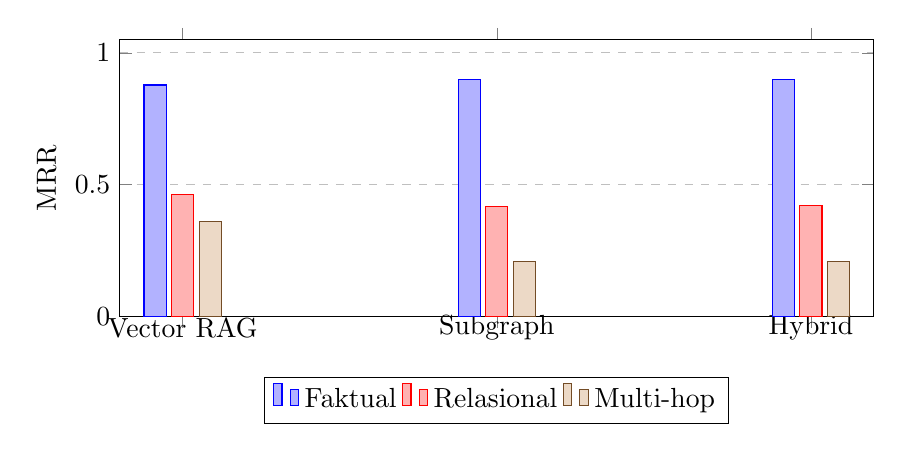
\begin{tikzpicture}
    \begin{axis}[
        ybar,
        width=0.92\textwidth,
        height=0.42\textwidth,
        bar width=8pt,
        ymin=0, ymax=1.05,
        ylabel={MRR},
        symbolic x coords={Vector RAG,Subgraph,Hybrid},
        xtick=data,
        x tick label style={rotate=0, anchor=center},
        legend style={at={(0.5,-0.22)}, anchor=north, legend columns=3},
        ymajorgrids=true,
        grid style=dashed,
    ]
        \addplot coordinates {(Vector RAG,0.8780) (Subgraph,0.9000) (Hybrid,0.9000)};
        \addlegendentry{Faktual}
        \addplot coordinates {(Vector RAG,0.4631) (Subgraph,0.4170) (Hybrid,0.4212)};
        \addlegendentry{Relasional}
        \addplot coordinates {(Vector RAG,0.3611) (Subgraph,0.2083) (Hybrid,0.2083)};
        \addlegendentry{Multi-hop}
    \end{axis}
    \end{tikzpicture}
    \caption{Perbandingan MRR mode retrieval pada setiap kategori pertanyaan}
    \label{fig:bab4-eval-mrr-category}
\end{figure}
